\section{Data Curation at Foundation-Model Scale}

\begin{frame}{}
    \LARGE Alignment and Post-Training: \textbf{Data Curation at Scale}

    \vspace{1em}
    \normalsize The raw pool is 240 trillion tokens. Which tenth do you keep, and how do you know it was the right tenth?
\end{frame}

\begin{frame}{From Common Crawl to a Training Set}
    \centering
    \begin{adjustbox}{max width=\linewidth}\begin{tikzpicture}[font=\small,
        st/.style={draw, rounded corners=2pt, minimum width=1.7cm, minimum height=0.9cm, align=center, fill=KAUSTcyan!15, font=\footnotesize},
        arr/.style={-{Stealth}, thick}]
        \node[st, fill=gray!12] (a) at (0,0) {Raw crawl\\{\scriptsize WARC}};
        \node[st] (b) at (2.0,0) {Extract\\{\scriptsize HTML to text}};
        \node[st] (c) at (4.0,0) {Language\\{\scriptsize fastText ID}};
        \node[st] (d) at (6.0,0) {Heuristics\\{\scriptsize repetition}};
        \node[st] (e) at (8.0,0) {Dedup\\{\scriptsize MinHash, exact}};
        \node[st, fill=darkorange!20] (f) at (10.0,0) {Quality\\{\scriptsize classifier}};
        \node[st, fill=gray!12] (g) at (12.0,0) {Mix\\{\scriptsize domains}};
        \draw[arr] (a) -- (b);
        \draw[arr] (b) -- (c);
        \draw[arr] (c) -- (d);
        \draw[arr] (d) -- (e);
        \draw[arr] (e) -- (f);
        \draw[arr] (f) -- (g);
        \node[font=\scriptsize, KAred] at (4.0,-0.85) {48\% of documents left};
        \node[font=\scriptsize, KAred] at (6.0,-0.85) {23\% left};
        \node[font=\scriptsize, KAred] at (8.0,-0.85) {about 10\% left};
    \end{tikzpicture}\end{adjustbox}
    \vspace{0.2em}
    \begin{itemize}\itemsep0.4em
        \item Stanford's CS336 calls data ``the most important thing to get right''. Labs keep it secret for competitive and copyright reasons, so what we know comes from open corpora.
        \item \textbf{Each stage earns points.} In RefinedWeb the zero-shot aggregate goes from 52.7 (raw) to 54.3 (filtered) to 56.2 (deduplicated).
        \item \textbf{Extraction is not a detail.} Re-extracting text from raw HTML beats the crawl's ready-made text files. In DCLM a better extractor alone adds about 2.5 points.
        \item One C4 rule, ``lines must end in punctuation'', removes about 30\% of all tokens.
    \end{itemize}
    \src{Retention figures: Penedo et al., ``The RefinedWeb Dataset for Falcon LLM,'' \href{https://arxiv.org/abs/2306.01116}{arXiv:2306.01116}, Table 4. Penedo et al., ``The FineWeb Datasets,'' \href{https://arxiv.org/abs/2406.17557}{arXiv:2406.17557}. Li et al., ``DataComp-LM,'' \href{https://arxiv.org/abs/2406.11794}{arXiv:2406.11794}. Liang, Stanford CS336 Lecture 13 (2025).}
\end{frame}

\begin{frame}{Deduplication: One Formula, One Surprise}
    \begin{columns}[T,onlytextwidth]
        \column{0.44\textwidth}
        \centering
        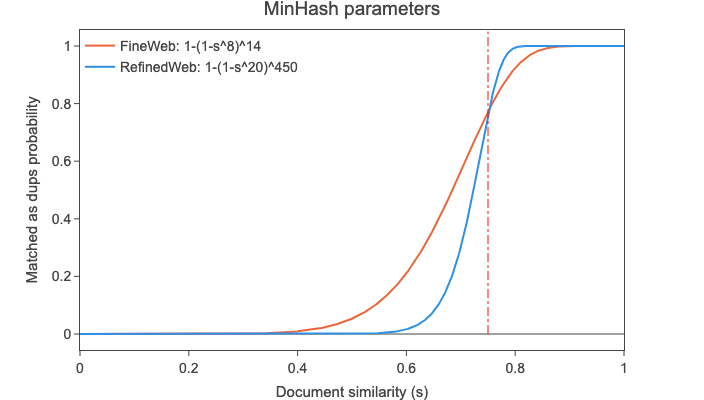
\includegraphics[width=\linewidth,height=0.4\textheight,keepaspectratio]{images/alignment-post-training/fineweb_minhash_params.png}
        \[
            P(s)=1-(1-s^{r})^{b}
        \]
        \column{0.54\textwidth}
        \begin{itemize}\itemsep0.4em
            \item \textbf{MinHash with banding.} With $b$ bands of $r$ rows, two documents of similarity $s$ become candidates with probability $P(s)$.
            \item FineWeb's $14\times 8$ catches a 75\%-similar pair 77\% of the time. RefinedWeb's $450\times 20$ cuts sharper, at far higher cost.
            \item \alert{The surprise.} Deduplicating \emph{across} all 96 crawl snapshots made models worse than deduplicating each one alone. In one old snapshot, the 10\% that global dedup kept trained \emph{worse} models than the 90\% it removed.
        \end{itemize}
    \end{columns}
    \vspace{0.3em}
    \takeaway{``Deduplicate more'' is not monotone. FineWeb2 later \emph{upsamples} by duplicate count.}
    \src{Leskovec, Rajaraman, Ullman, \emph{Mining of Massive Datasets}, Ch. 3. Figure and results: Penedo et al., FineWeb paper and blog, \href{https://arxiv.org/abs/2406.17557}{arXiv:2406.17557}, Figure 5. Penedo et al., ``FineWeb2,'' \href{https://arxiv.org/abs/2506.20920}{arXiv:2506.20920}.}
\end{frame}

\begin{frame}{Model-Based Filtering, and Its Hidden Cost}
    \begin{columns}[T,onlytextwidth]
        \column{0.43\textwidth}
        \centering
        \small
        \begin{adjustbox}{max width=\linewidth}\begin{tabular}{lc}
            \toprule
            \textbf{DCLM filter (1B model)} & \textbf{Core} \\
            \midrule
            PageRank & 26.1 \\
            AskLLM & 28.6 \\
            Perplexity filter & 29.0 \\
            Top-$k$ average logits & 29.2 \\
            \rowcolor{KAUSTcyan!12} fastText classifier & 30.2 \\
            \bottomrule
        \end{tabular}\end{adjustbox}

        \vspace{0.5em}
        {\scriptsize The winner is a simple fastText classifier trained on about 400k documents. The resulting 7B model is comparable to Llama 3 8B on MMLU with 6.6$\times$ less compute.}
        \column{0.55\textwidth}
        \begin{itemize}\small\itemsep0.3em
            \item \textbf{DCLM} fixes the model and training recipe and varies only the data. It keeps about 10\% of a 240T-token pool.
            \item \textbf{FineWeb-Edu.} An LLM scores educational value from 0 to 5. A small regressor on embeddings copies the scores to the whole corpus. MMLU 33 to 37\%, ARC 46 to 57\%. It matches the Matrix corpus on MMLU with almost 10$\times$ fewer tokens.
            \item \textbf{What counts as quality?} DCLM's positive examples are instruction data and top ELI5 posts. ``Quality'' partly means ``looks like what benchmarks reward''.
        \end{itemize}
    \end{columns}
    \begin{itemize}\itemsep0.4em
        \item \textbf{The cost shows at long horizons.} Keeping 10\% leaves too few unique tokens for a 15T-token run. Nemotron-CC ensembles three classifiers (their top picks overlap by only 10.1\%), keeps the lower tiers too, and adds 1.9T tokens of \emph{rephrased} text. Result: four times more unique real tokens, and MMLU 59.0 against 53.4.
    \end{itemize}
    \src{Li et al., ``DataComp-LM,'' \href{https://arxiv.org/abs/2406.11794}{arXiv:2406.11794}, Table 4 and abstract. Penedo et al., \href{https://arxiv.org/abs/2406.17557v2}{arXiv:2406.17557v2}, Section 4. Su et al., ``Nemotron-CC,'' ACL 2025, \href{https://arxiv.org/abs/2412.02595}{arXiv:2412.02595}.}
\end{frame}

\begin{frame}{How Much of Each Domain? Mixing Becomes a Law}
    \begin{columns}[T,onlytextwidth]
        \column{0.5\textwidth}
        \begin{itemize}\itemsep0.4em
            \item \textbf{DoReMi.} A small proxy upweights the domains where it trails a reference model most.
            \item Its answer on The Pile: web text from 0.11 to \alert{0.61}, arXiv from 0.105 to 0.004.
            \item \textbf{Data mixing law.} Validation loss on domain $i$ is exponential in the mixture proportions $r_j$:
            \[
                L_i(r_{1\ldots M})=c_i+k_i\exp\Big(\sum_{j=1}^{M}t_{ij}\,r_j\Big)
            \]
        \end{itemize}
        \column{0.48\textwidth}
        \centering
        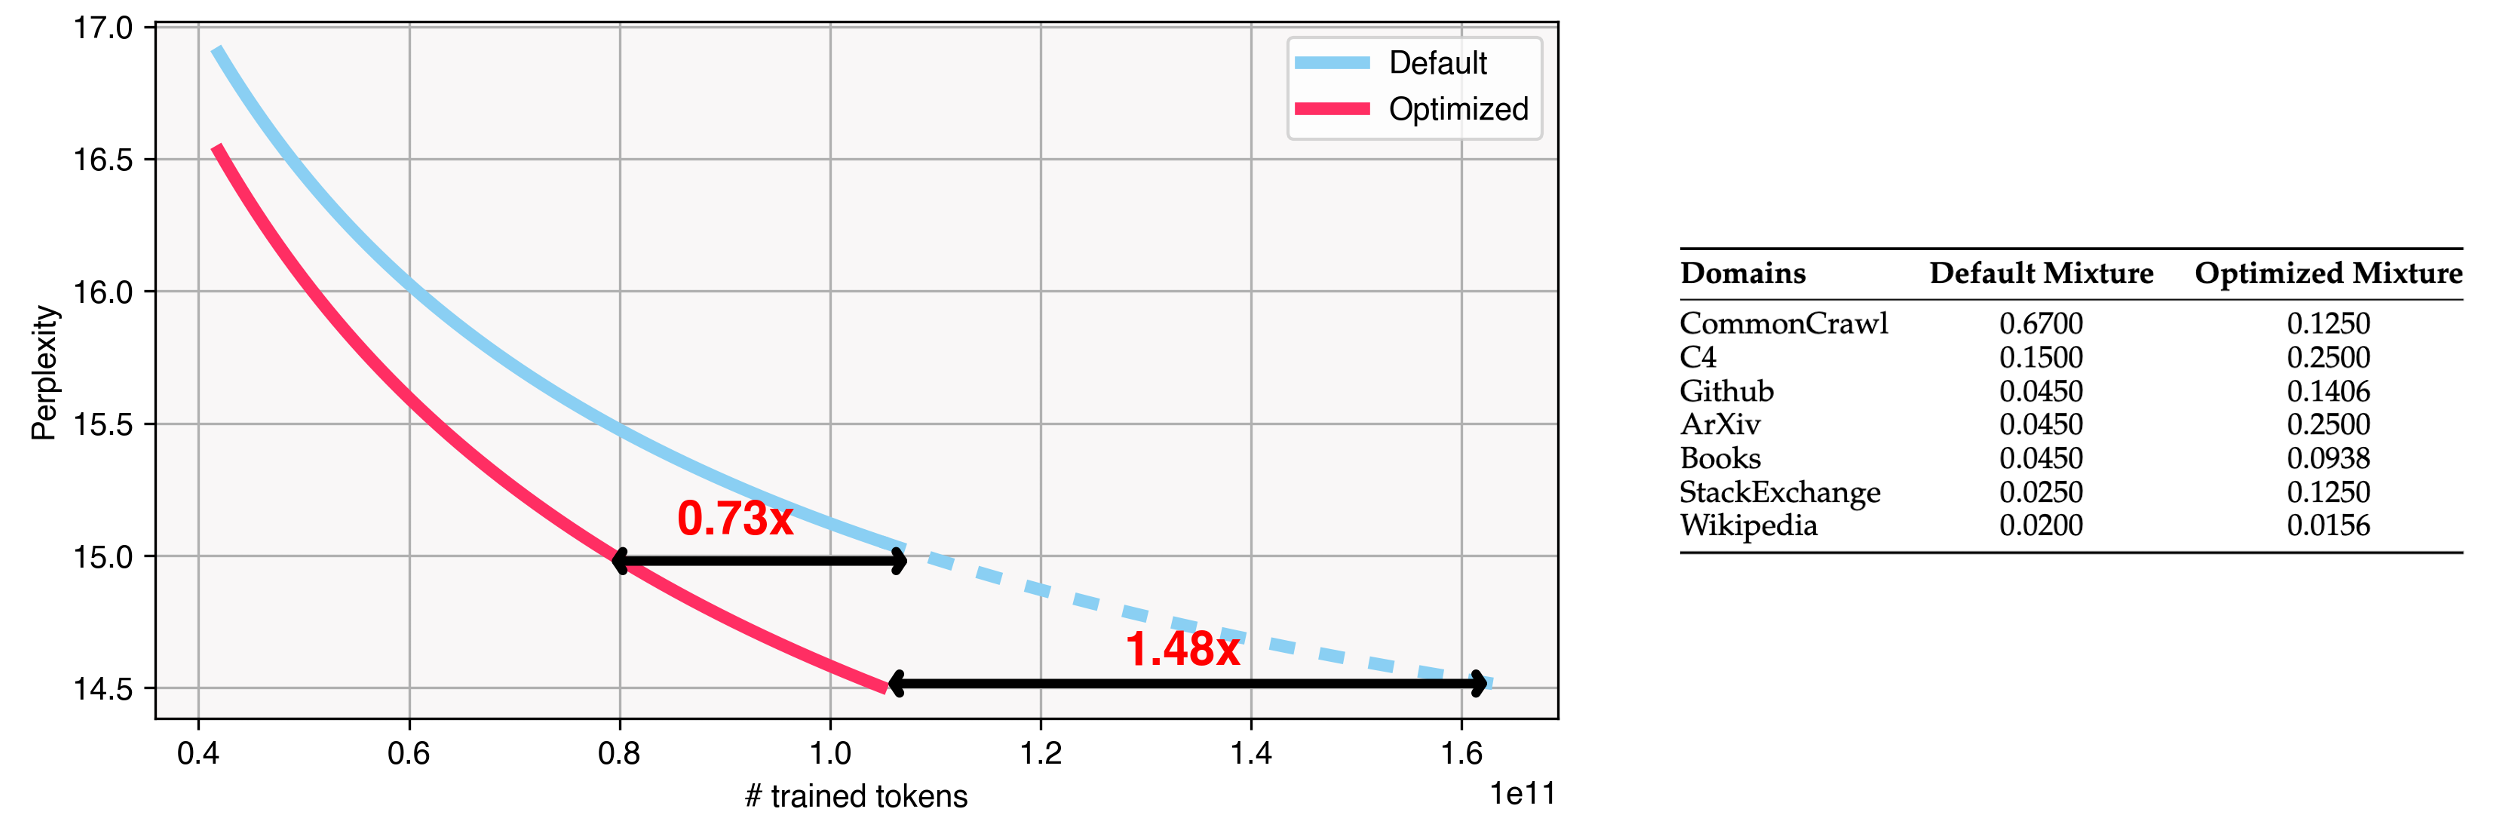
\includegraphics[width=\linewidth,height=0.34\textheight,keepaspectratio]{images/alignment-post-training/dml_fig8_optimised_mixture.png}

        \vspace{0.3em}
        {\scriptsize The predicted mixture reaches the default's loss in 0.73 of the steps, worth 1.48 times more training.}
    \end{columns}
    \vspace{0.3em}
    \takeaway{Automated mixing moves weight \emph{toward} diverse web text. RegMix agrees: web corpora predict downstream performance best.}
    \src{Xie et al., ``DoReMi,'' NeurIPS 2023, \href{https://arxiv.org/abs/2305.10429}{arXiv:2305.10429}. Ye et al., ``Data Mixing Laws,'' ICLR 2025, \href{https://arxiv.org/abs/2403.16952}{arXiv:2403.16952}, Eq. 7 and Figure 8. ``RegMix,'' ICLR 2025, \href{https://arxiv.org/abs/2407.01492}{arXiv:2407.01492}.}
\end{frame}

\begin{frame}{Mid-Training: The Stage Between Pre- and Post-}
    \begin{columns}[T,onlytextwidth]
        \column{0.4\textwidth}
        \centering
        \small
        \begin{adjustbox}{max width=\linewidth}\begin{tabular}{lr}
            \toprule
            \textbf{Llama 3 pre-training mix} & \\
            \midrule
            General knowledge & 50\% \\
            Maths and reasoning & 25\% \\
            Code & 17\% \\
            Multilingual & 8\% \\
            \bottomrule
        \end{tabular}\end{adjustbox}

        \vspace{0.8em}
        \begin{adjustbox}{max width=\linewidth}\begin{tabular}{lcc}
            \toprule
            \textbf{OLMo 2, GSM8K} & \textbf{before} & \textbf{after} \\
            \midrule
            7B & 24.1 & 67.5 \\
            13B & 37.3 & 75.1 \\
            \bottomrule
        \end{tabular}\end{adjustbox}
        \column{0.58\textwidth}
        \begin{itemize}\itemsep0.45em
            \item Data now comes in three stages: pre-training for \textbf{volume}, mid-training for \textbf{targeted quality}, post-training for the small and best.
            \item \textbf{Annealing (Llama 3).} Decay the learning rate to zero while upsampling high-quality data. GSM8K rises by 24.0\% for the 8B model. For 405B the gain is negligible.
            \item \textbf{OLMo 2.} Stage 1 is 3.9T tokens, over 95\% web. Stage 2 is 50B to 300B tokens of the top-filtered web, instruction data and maths. Several runs with different data orders are then \emph{averaged in weight space}.
        \end{itemize}
    \end{columns}
    \vspace{0.3em}
    \takeaway{Mid-training is now a named stage. Its gains are largest for small models.}
    \src{Meta, ``The Llama 3 Herd of Models,'' \href{https://arxiv.org/abs/2407.21783}{arXiv:2407.21783}. Team OLMo, ``2 OLMo 2 Furious,'' \href{https://arxiv.org/abs/2501.00656}{arXiv:2501.00656}, Table 9. Ai2, Olmo 3 announcement (2025). Liang, Stanford CS336 Lecture 13 (2025).}
\end{frame}

\begin{frame}{Decontamination: Overlap Is Not Impact}
    \begin{columns}[T,onlytextwidth]
        \column{0.5\textwidth}
        \textbf{What n-grams miss}
        \begin{center}
        \small
        \begin{adjustbox}{max width=\linewidth}\begin{tabular}{lcc}
            \toprule
            \textbf{Llama-2-13B} & \textbf{clean} & \textbf{rephrased test set} \\
            \midrule
            MMLU & 54.8 & 89.9 \\
            HumanEval & 36.0 & 81.1 \\
            GSM8K & 28.7 & 95.3 \\
            \bottomrule
        \end{tabular}\end{adjustbox}
        \end{center}
        \begin{itemize}\itemsep0.3em
            \item Fine-tune on \emph{rephrased} test items and scores explode. N-gram detection scores an F1 of 0 on translated items.
            \item Fix: retrieve by embedding, then let an LLM judge semantic equivalence.
        \end{itemize}
        \column{0.48\textwidth}
        \textbf{What n-grams over-count}
        \begin{itemize}\itemsep0.3em
            \item Measure the effect, not the overlap:
            \[
                \mathrm{EPG}=\mathrm{Perf}(\text{full})-\mathrm{Perf}(\text{clean subset})
            \]
            \item Llama 3: Natural Questions is 52\% contaminated with ``virtually no effect''. BIG-Bench Hard is 95\% flagged with estimated gains of 26 to 41 points.
            \item DCLM: removing MMLU overlaps did not lower the score.
        \end{itemize}
    \end{columns}
    \vspace{0.3em}
    \takeaway{Report the rule (T\"ulu 3: 8-grams covering over 50\% of a test item), the removal rate per dataset, and an ablation with and without.}
    \src{Yang et al., ``Rethinking Benchmark and Contamination for Language Models with Rephrased Samples,'' \href{https://arxiv.org/abs/2311.04850}{arXiv:2311.04850}. Singh et al., \href{https://arxiv.org/abs/2411.03923}{arXiv:2411.03923}. Llama 3, \href{https://arxiv.org/abs/2407.21783}{arXiv:2407.21783}, Table 15 (BBH row reconstructed from the PDF, verify before citing).}
\end{frame}

\begin{frame}{Curating Post-Training Data: Thousands, Not Millions}
    \begin{center}
    \small
    \begin{adjustbox}{max width=\linewidth}\begin{tabular}{l>{\raggedright\arraybackslash}p{5.3cm}>{\raggedright\arraybackslash}p{5.6cm}}
        \toprule
        \textbf{Method} & \textbf{Selection signal} & \textbf{Result} \\
        \midrule
        LIMA & 1,000 hand-curated pairs & 65B model preferred or tied against GPT-4 in 43\% of cases \\
        AlpaGasus & an LLM grades each example & 9k of 52k beats the full set, 5.7 times faster \\
        IFD & how much the instruction helps predict the answer & 5\% of Alpaca beats the full set \\
        Deita & complexity, quality and diversity & 6k samples, MT-Bench 7.55 with DPO \\
        \bottomrule
    \end{tabular}\end{adjustbox}
    \end{center}
    \[
        \mathrm{IFD}_\theta(Q,A)=\frac{s_\theta(A\mid Q)}{s_\theta(A)}
        \qquad\text{(loss on the answer with the instruction, over loss without it)}
    \]
    \begin{itemize}\itemsep0.4em
        \item LIMA calls this the \textbf{superficial alignment hypothesis}. CS336's version: SFT works best when \emph{extracting} pre-training behaviours, not adding new ones.
    \end{itemize}
    \src{Meta, ``LIMA: Less Is More for Alignment,'' \href{https://arxiv.org/abs/2305.11206}{arXiv:2305.11206}. Chen et al., ``AlpaGasus,'' \href{https://arxiv.org/abs/2307.08701}{arXiv:2307.08701}. Li et al., ``From Quantity to Quality,'' NAACL 2024, \href{https://arxiv.org/abs/2308.12032}{arXiv:2308.12032}. ``Deita,'' ICLR 2024, \href{https://arxiv.org/abs/2312.15685}{arXiv:2312.15685}. Hashimoto, CS336 Lecture 15 (2025).}
\end{frame}

\begin{frame}{The Quality-Consent Squeeze}
    \begin{itemize}\itemsep0.45em
        \item \textbf{Provenance.} Fewer than 33\% of datasets carry a restrictive licence. Yet over \alert{80\%} of their \emph{source content} has non-commercial restrictions.
        \item \textbf{Consent.} In one year, 28\% or more of the most critical sources in C4 became fully restricted by robots.txt. These are the maintained sites a quality classifier prefers.
    \end{itemize}
    \begin{center}
    \small
    \begin{adjustbox}{max width=\linewidth}\begin{tabular}{>{\raggedright\arraybackslash}p{3.6cm}>{\raggedright\arraybackslash}p{9.7cm}}
        \toprule
        Bartz v. Anthropic (Jun 2025) & training on purchased, scanned books was fair use. Over 7M pirated copies were not. Settled for 1.5 billion dollars \\
        Kadrey v. Meta (Jun 2025) & judgment for Meta on 13 authors' books, but the court expects unlicensed training to be illegal ``in most cases'' \\
        EU code of practice (Jul 2025) & obey robots.txt, exclude persistently infringing sites, publish a summary of training content with top domains \\
        \bottomrule
    \end{tabular}\end{adjustbox}
    \end{center}
    \takeaway{How data was \emph{acquired} can cost billions even when training on it is lawful.}
    \src{Longpre et al., ``Bridging the Data Provenance Gap,'' \href{https://arxiv.org/abs/2412.17847}{arXiv:2412.17847}, and ``Consent in Crisis,'' \href{https://arxiv.org/abs/2407.14933}{arXiv:2407.14933}. Kadrey v. Meta, N.D. Cal., order of 25 Jun 2025. Bartz details via that order and Wikipedia (secondary). GPAI Code of Practice, Copyright chapter.}
\end{frame}

\begin{frame}{Data Curation: What to Remember}
    \begin{itemize}\itemsep0.45em
        \item The pipeline is extract, identify language, filter, deduplicate, classify, mix. \textbf{Every stage is worth points}, including the HTML extractor.
        \item A cheap classifier picks the top 10\% well. At long horizons that 10\% is too little, and the answer is \textbf{ensembles plus rephrasing}.
        \item Mixing can be predicted from small runs. The predictions favour \textbf{diverse web text}.
        \item Contamination must be measured by \textbf{impact}. N-grams both miss rephrased items and over-count harmless overlap.
        \item 2026: learned curation. A single 0.6B model that keeps, edits, deletes or rewrites each page replaces the heuristic stages.
    \end{itemize}
    \vspace{0.3em}
    \takeaway{\textbf{Next.} We have an optimiser, a reward, and data pipelines that the model itself can run. What happens if we connect them and remove the human?}
    \src{Yu et al., ``ReScraper,'' \href{https://arxiv.org/abs/2609.34287}{arXiv:2609.34287} (abstract).}
\end{frame}
